\section{Tábua de Logaritmo}

A despeito da ciência e tecnologia hodierna terem evoluído o bastante para computar $4538 \cdot 675$ instantanemente, até a década de 1970 tal produto era trabalhoso e exigia o uso de métodos com aplicação dos logaritmos, vulgo as tábuas de logaritmos e as réguas de cálculo.


\begin{figure}[H]
    \centering
    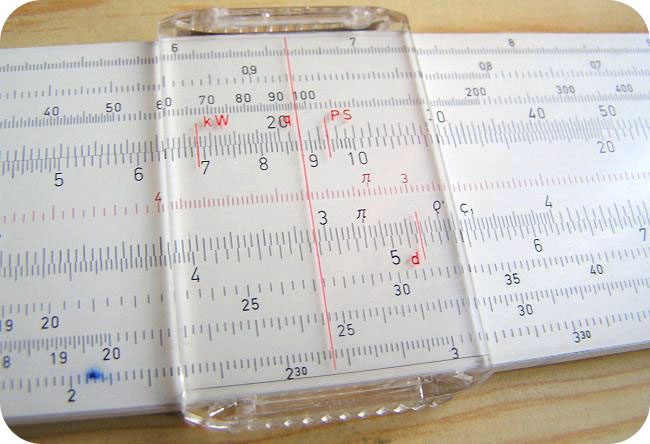
\includegraphics[height=6cm]{img/regua.png}
    \caption{Régua de Cálculo}
\end{figure}

Assim, mostraremos como se utilizar a tábua de logaritmo para calcular produtos, utilizemos como exemplo $4538\cdot 675$. Primeiramente, um pouco de teoria, temos que:

\begin{align*}
    & a\cdot b \\ 
    & \implies \log (a\cdot b) = \log (a) + \log (b)\\ 
    & \implies a\cdot b = \log ^{-1} (\log (a) + \log (b))
\end{align*}



\begin{figure}[H]
    \centering
    
\includegraphics[height=9cm]{img/tabua.png}
    \caption{Capa do Arithmetica Logarithmica}
\end{figure}






3,656864




\subsection{Algoritmos}

\subsection{Raízes Quadradas}x 




\subsection{Atalhos e logaritmos dos primeiros primos}
\subsection{O uso das diferenças finitas}
\subsection{Nuemros Primos}


